%!TEX root=../Vorlage_DA.tex
%	########################################################
% 				Projektbeschreibung
%	########################################################


%	--------------------------------------------------------
% 	Überschrift, Inhaltsverzeichnis
%	--------------------------------------------------------
\chapter{Interpreter}


%	--------------------------------------------------------
% 	Allgmeine Hinweise
%	--------------------------------------------------------
\section{Allgemeiner Teil (Theorie)}

\subsection{Aufbaumöglichkeiten eines Interpreters}

\subsubsection{Bytecode Interpreter}
Bei der Compilierung wird eine Zwischensprache erzeugt, welche aus einer Sammlung von Befehlen besteht. Dadurch wird das System
betriebssystemunabhängig und der Code ist nahezu hardwareunabhängig.

Jedoch muss zum Ausführen des Programmes, welches in die Zwischensprache übersetzt wurde, eine virtuelle Maschine vorhanden sein.
Dadurch, dass während der Ausführung des Programmes compiliert werden muss, sinkt die Geschwindigkeit gegenüber
nativ compilierten Programmen.

%Durch die Verwendung des Just-in-time-compilation Verfahrens kann die Geschwindigkeit wieder verbessert werden.

\subsubsection{Abstrakter Syntaxbaum Interpreter}
Bei dem von uns gewählten Ansatz wird der Quellcode in einen optimierten abstrakten Syntaxbaum übersetzt. Dieser Baum wird während der Laufzeit
abgearbeitet. Jeder Knoten muss nur einmal durchsucht werden. Im Vergleich zu einem Bytecode wird beim Abstrakten Syntaxbaum die Struktur
des Programmes beibehalten. Dadurch kann man Fehler im Programm leichter analysieren.

%\subsubsection{Just-in-time compilation}
%Um Plattformunabhängigkeit gewährleisten zu können, ist es notwendig, gewisse Teile während der Laufzeit zu kompilieren. 
%Darunter leidet aber die Ausführungsgeschwindigkeit. Deshalb wurde ein Verfahren entwickelt, welches versucht,
%diesen Nachteil zu lindern.

%Während der Anwendung des Programmes wird ein lauffähiger Maschinencode erzeugt. Es werden hierbei oft verwendete Programmteile
%während der Laufzeit kompiliert und für einen späteren Gebrauch zwischengespeichert. Hierbei ist es wichtig, dass die Compilation nicht
%zu aufwendig ist, da sonst die Geschwindigkeit des Programmes darunter leiden könnte.

\subsection{Call Stack}
Der sogenannte Call Stack, auch Aufrufstapel genannt, enthält während der Laufzeit Informationen über die gerade ablaufenden 
Unterprogramme. 

%Der Call Stack wird mit einem Befehlssatz zum Befüllen, Abbauen und zum Wiedereintritt in ein anderes Unterprogramm bearbeitet.

Sobald mehrere Threads oder Prozesse ausgeführt werden sollen, muss für jeden gewünschten Prozess ein eigener Call Stack eingerichtet
werden, damit sich die Variablen und Rücksprungadressen nicht überschreiben.

\subsubsection{Lokale Variablen}
Wenn lokale Variablen verwendet werden, wird am Call Stack der nötige Variablenspeicher reserviert. Da jeder Aufruf seine
eigenen Variablen hat, sind rekursive Unterprogrammaufrufe möglich. Um vom aktuellen Aufruf auf den letzten zurückzukommen, ist
es notwendig, eine Referenzadresse auf den letzten Aufruf zu speichern.


%	--------------------------------------------------------
% 	Lösungsansätze
%	--------------------------------------------------------
%\section{Lösungsansätze}
%	--------------------------------------------------------
% 	Realisierte Lösungen
%	--------------------------------------------------------
\section{Realisierte Lösungen}
Hier wird der Aufbau des Interpreters näher erläutert und die einzelnen Funktionen werden näher vorgestellt.

Der Interpreter wurde genauso wie die anderen Komponenten in Java implementiert.
Am meisten wurde beim Aufbau des Interpreters auf die Schnittstelle zum GUI geachtet, da der Interpreter für eine einfachere
Programmdarstellung optimiert werden sollte.

Der Aufbau des Abstrakten Syntaxbaumes ist im Kapitel Compiler zu finden. Dort werden die einzeln verwendeten 
Knoten näher erläutert.

\subsection{Memory}
Hier wird das Speichermodell und deren Anforderungen an den Interpreter näher erläutert.
Ein wichtiger Teil des Speichermodells ist die Aufbewahrung von einzelnen Variablen.

\subsubsection{Aufbau unseres Stack Frames}
\begin{figure}[Stack Frame]
\begin{center}
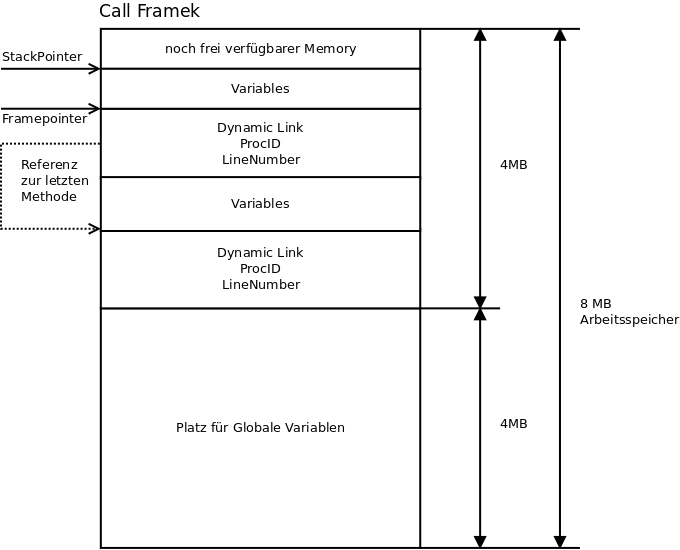
\includegraphics[width=0.9\textwidth]{./media/images/interpreter/memory/stackframe.png}
\label{stackframe1} 
\caption{Aufbau des von uns verwendeten Stack Frames}
\end{center}
\end{figure}
%--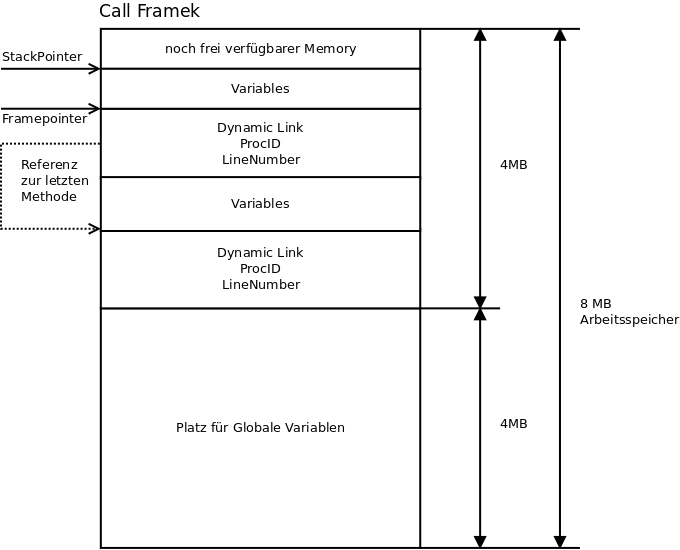
\includegraphics[scale=0.3]{./media/images/interpreter/memory/stackframe.png}

\subsection{Aufbau des Memorys}
Da wir für unser Projekt nicht sehr viel Arbeitsspeicher benötigen, wurden 8 MB Arbeitsspeicher für den Memory reserviert.
Wie man in \ref{stackframe1} erkennen kann, wurde dieser in 2 Hälften geteilt, wovon der untere Teil für globale Variablen
und der obere Teil für Methoden verwendet wird.


\subsubsection{Aufruf einer neuen Methode}
\begin{enumerate}
 \item Die Zeilennummer wird in den Speicher geschrieben (Größe von 4 Byte)
 \item Der Methodenname wird im Speicher vermerkt (Größe von 4 Byte)
 \item Eine Referenz des Framepointers, mit welcher man zum letzten Methodenaufruf zurückgelangen kann, wird im Speicer notiert (Größe von 4 Byte)
 \item Nun wird der Framepointer auf\footnote{Untere Referenzadresse im Memory} denselben Wert wie der Stackpointer{Obere Referenzadresse im Memory} gesetzt.
 \item Um genügend Speicher für Variablen gewährleisten zu können, muss nun zum StackPointer die vom Compiler vorgegebene Variablengröße
 hinzugefügt werden. Dort werden dann alle lokalen Variablen zwischengespeichert.
\end{enumerate}
 
\subsubsection{Schließen einer Methode}
\begin{enumerate}
 \item Der Stackpointer wird auf Framepointer gesetzt (Variablen werden entfernt).
 \item Um an den Startwert der Referenz zu gelangen müssen nun vom Stackpointer 4 Bytes abgezogen werden.
 \item Die Referenz verweißt auf den im letzten Methodenaufruf verwendeten Framepointer. Somit wird der Framepointer nun mit dem Wert
 der Referenz versehen.
 \item Um den richtigen Stackpointer zu bekommen, ist es nun notwendig den Stackpointer um den vorherigen Methodennamen und um die vorher verwendete Zeilennummer zu veringern.
 Somit muss der Stackpointer um 8 Byte veringert werden.
\end{enumerate}

\subsubsection{Speicherverwaltung}
Da bei der Speicherverwaltung viele Fehler auftreten könnten, ist es wichtig, dass diese mit verschiedensten Exceptions abgefangen werden.

Die statische Klasse Memory beinhaltet alle Funktionen, welche für den Interpreter notwenig sind.

Es werden verschiedene Datentypen unterstützt:
\begin{itemize}
 \item int - 4 Byte
 \item float - 4 Byte
 \item char - 2 Byte 
 \item boolean - 1Byte
 \item string - 4 Byte
\end{itemize}

Hierbei sind die Bytegrößen zu beachten, wobei bei dem Datentyp String nur die Stringadresse gespeichert wird. Alle Variablen können
mit der nötigen Adresse und der zum Variablennamen passenden Funktion abgefragt werden.

\subsection{Interpreter}
Weil wir eine einfache Darstellung der aktuellen Variablen bezweckten und den Ablauf des Programmes nicht verändern wollten, kam für 
uns nur der Abstrakte Syntaxbaum-Interpreter in Frage.

Es wurden einige Vorgaben gemacht, um ein Zusammenarbeiten zwischen Compiler und Interpreter möglich zu machen. Somit wurde eine gewisse
Baumstruktur vorgegeben. In diesem konnten die Knoten nur in einer bestimmten Reihenfolge auftreten.

\subsection{Statements}
\subsubsection{assign}
Bei einem Assign wird eine bestimmte Variable in den Memory geschrieben. Bevor dies jedoch geschehen kann, ist es notwendig,
den Datentyp herauszufinden. Dafür wird der Typ des rechten Knotens geprüft.

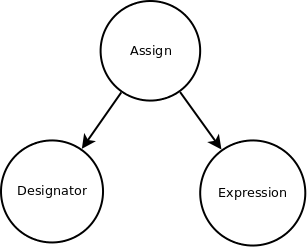
\includegraphics[width=0.4\textwidth]{./media/images/interpreter/syntaxbaum/statements/assign.png}

\subsubsection{startsequenz}
Mithilfe der Startsequenz wird das derzeitige Unterprogramm abgearbeitet.

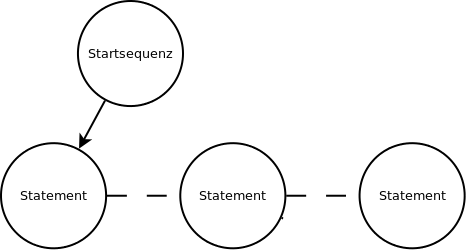
\includegraphics[width=0.6\textwidth]{./media/images/interpreter/syntaxbaum/statements/startsequenz.png}

\subsubsection{trap}
Die Trap wird dazu benötigt, um einen Unterprogrammaufruf, welcher keine Rückgabeparameter besitzt, zu beenden.

\subsubsection{if}
Auf der linken Seite des Knotens stehen die Bedingungen, auf der rechten Seite steht das auszuführende Programm, wenn die Bedingung
true ergibt.

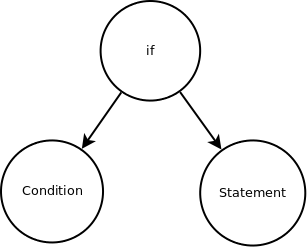
\includegraphics[width=0.4\textwidth]{./media/images/interpreter/syntaxbaum/statements/if.png}

\subsubsection{Ifelse}
Das Ifelse ist grundsätzlich genauso aufgebaut wie das If. Der wesentliche Unterschied besteht darin, dass, sobald die Condition
false ergibt, die andere if-Funktion abgearbeitet wird.

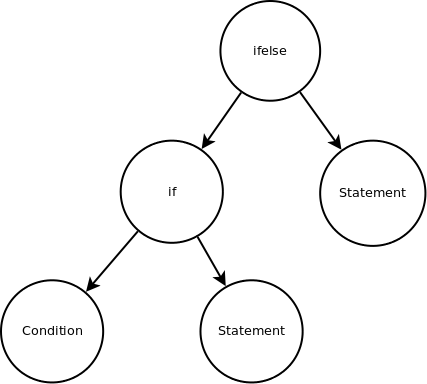
\includegraphics[width=0.4\textwidth]{./media/images/interpreter/syntaxbaum/statements/ifelse.png}

\subsubsection{while}
Sie funktioniert ähnlich wie ein If, das Statement jedoch wird so oft wiederholt, bis die Condition false ergibt.

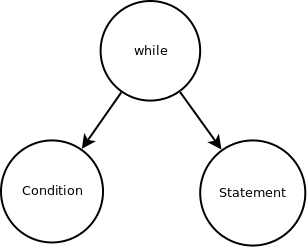
\includegraphics[width=0.4\textwidth]{./media/images/interpreter/syntaxbaum/statements/while.png}

\subsection{call}
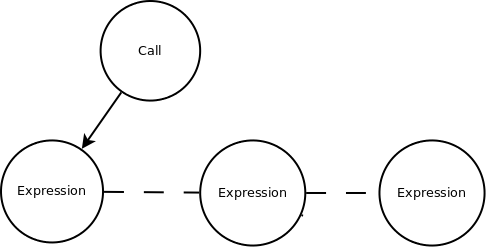
\includegraphics[width=0.6\textwidth]{./media/images/interpreter/syntaxbaum/statements/call.png}

Ein Call Knoten hat mehrere Funktionen. Die Richtige wird anhand des Namens herausgefunden. Dies sind schon vordefinierte
Funktionsnamen, welche in einem Programm nicht erneut verwendet werden können.

Hier eine Auflistung dieser Funktionen:

\subsubsection{print}
Hiermit wird ein Char-Zeichen dem StdInOut Interface übergeben. Somit kann dieses danach vom GUI ausgeben werden.

\subsubsection{read}
Wenn Read aufgerufen wird, werden vom Interface StdInOut Char-Variablen eingelesen und diese als Return Wert gesetzt.

\subsubsection{length}
Hier kann man die Länge eines Strings bestimmen lassen, dieser wird wiederum als Return-Wert gesetzt.

\subsubsection{time}
``time'' dient zum Bestimmen der Zeit, welche wiederum als Return-Wert zurückgegeben wird.

\subsubsection{Normaler Aufruf}
Sobald ein Aufruf erfolgt, werden alle Variablen, welche übergeben werden sollen, in einem Objekt zwischengespeichert. Nun kann ein
neues Memoryframe geöffnet werden. Die Variablen, welche in einem Objekt zwischengespeichert wurden, können nun in das neue
Memoryframe übertragen werden.

Nun wird eine Startsequenz ausgeführt, damit der Unterprogrammaufruf abgearbeitet werden kann.

\subsection{Designators}
Auf Designators werden bestimmte Werte gespeichert. Weiters sind sie für die richtige Zuweisung der Adresse notwendig.
Hier wird in 3 Grundtypen unterschieden:

\subsubsection{Ident}
Wenn ein Ident aufgerufen wird, werden verschiedene Faktoren geprüft.
\begin{itemize}
 \item Falls der Identifer global ist, wird der Globalpointer mit der Objektadresse addiert.
 \begin{lstlisting}[language=JAVA]
 adr = Memory.getGlobalPointer() + obj.adr;	
  \end{lstlisting}
  Trifft voriges nicht zu, wird anstatt des Globalpointers der Framepointer des aktuellen Aufrufes zur Objektadresse addiert.
   \begin{lstlisting}[language=JAVA]
 adr = Memory.getFramePointer() + obj.adr;
  \end{lstlisting}
 \item Wenn der Identifer eine Referenz auf eine Adresse ist, wird hier die gespeicherte Adresse geladen.
\end{itemize}



\subsubsection{Dot}
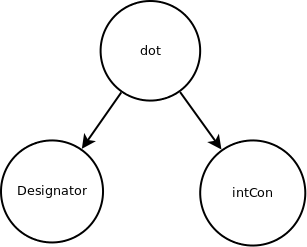
\includegraphics[width=0.4\textwidth]{./media/images/interpreter/syntaxbaum/designators/dot.png}

Dieser Knoten wird für Strukturen angewandt. Um die richtige Adresse für eine Variable in der Struktur zu bekommen, muss die Adresse des linken
Knotens mit der rechten Seite des Knotens addiert werden.

\begin{lstlisting}[language=JAVA]
return Adr(p.left) + p.right.val
\end{lstlisting}

\subsubsection{Index}
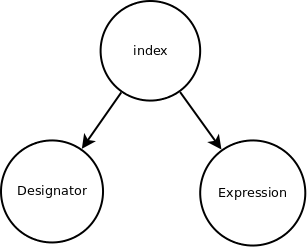
\includegraphics[width=0.4\textwidth]{./media/images/interpreter/syntaxbaum/designators/index.png}

Um den Index auszurechnen, ist es notwendig, die Expression auf der rechten Seite aufzulösen.
Nun kann die Adresse berechnet werden. Diese setzt sich aus dem Produkt der Adresse des rechten Knotens und der Größe der Indexelemente zusammen.

\begin{lstlisting}[language=JAVA]
return Adr(p.left) + p.left.type.elemType.size * index;
\end{lstlisting}

\subsection{Expressions}
Expressions werden grundsätzlich für Berechnungen und Typconvertierungen verwendet, aus diesem Grund ist es wichtig, dass jeder Datentyp seine
eigene Expressions-Methode besitzt.

\subsection{Conditions}
Conditions werden zur Verwendung von if-Bedingungen und für Schleifen benötigt.

%	--------------------------------------------------------
% 	Kalkulation
%	--------------------------------------------------------
\section{Kalkulation}


%	--------------------------------------------------------
% 	Arbeitseinteilung
%	--------------------------------------------------------
\section{Arbeitseinteilung}